% !TeX root = ../../../main.tex

As it has been explained in the previous section, a theory map, i.e.\ an
\fktab, is made of two main components: a \pdf independent interpolation
\textit{grid} and an \textit{evolution operator}.

For the second one, we just need a single provider, able to compute the \dglap
solving operator for a variety of theory settings (corresponding to different
\pdf fits, e.g.\ \nlo and \nnlo \qcd evolution), able to perform the
operator computation as efficient as possible, and to smoothly interface with
the grid for convolution.
Multiple evolution codes are already available for the purpose
\cite{Vogt:2004ns,Salam:2008sz,Botje:2010ay,Bertone:2013vaa,Bertone:2017gds},
but when the authors decided to begin the full rework of the architecture, it
has been clear that a dedicated tool, with this exact goal in mind, would have
been an ideal solution.
For this reason, the software package \eko \cite{Candido:2022tld} has been
created, providing a framework to solve \dglap equations in Mellin space,
similarly to \cite{Vogt:2004ns}, but generating an output in $x$-space, i.e.\
the one usually employed by the fit.
Moreover, while not being the first tool to provide evolution operators
\cite{Bertone:2013vaa,Salam:2008sz}, it produces them as the default output,
optimizing the process as much as possible, storing them in a dedicated file
format, designed to be easily available from different programming languages.


\eko is very different from \apfel, the tool on which the NNPDF framework has
until now relied. For instance \apfelgrid (then \apfelcomb), the tool which
generates \apfel-based \fktab, introduces an explicit dependency on \apfel
itself (and thus its internals).
\eko instead not only exposes a restricted public API (making all the dependent
projects decoupled from its very internals), but the dependency is not required
at all to consume the \eko output, consisting of float arrays stored in a very
common \href{https://en.wikipedia.org/wiki/Tar\_(computing)}{\texttt{tar}}
archive, and standard \href{https://yaml.org/}{\texttt{YAML}} metadata.
On the other side, the observable grids have to be produced by different
generators, in order to cover the full variety of available processes.
For this reason, we need an interface to them, with the following targets:
standardizing the output and making it reproducible.

The solution we propose is thus based on the concept of interpolation grid, and
specifically on \pineappl as an interface.
In particular, \pineappl exposes APIs to different languages: it is natively
written in Rust, but has an API to C/C++, that can be consumed also by a
Fortran application (examples provided for all of them), and a Python API,
mostly dedicated to scripting and integration with the rest of the pipeline,
but there are providers (essentially \yadism
\cite{candido_alessandro_2022_6285149}, used for DIS at NNLO) already using it
to fill grids.

Since different generators require different inputs, we are trying to
standardize them into a common format for which other cards can be generated,
called \textit{pinecard}.
This is still work in progress, nevertheless, it is useful to speak of
pinecards, since they are used as inputs for \pinefarm, that is the unique
Python package working as a front-end for the various generators.
Essentially, each generator needs dedicated code to run, but this interface has
to be written once, and then is part of \pinefarm, standardizing the input for
that generator, and part of the input across all of them (e.g.\ metadata, like
references and observable details, or theory parameters).
In \cref{fig:pine/pineline} we summarize our architecture: the generators are
directly interfaced with the \pineappl library, and the output is thus
standardized to an interpolation grid (for one or two colliding hadrons), the
input instead consists of a \textit{pinecard}.

Once the grid is available, \pineko (a package dedicated to the final
construction of \fktab{}s) can extract the details of the operator needed for
the \fktab generation from the grid, generate the \eko input, and then combine
the grid and the operator into the final \fktab.

\begin{figure}
  \centering
  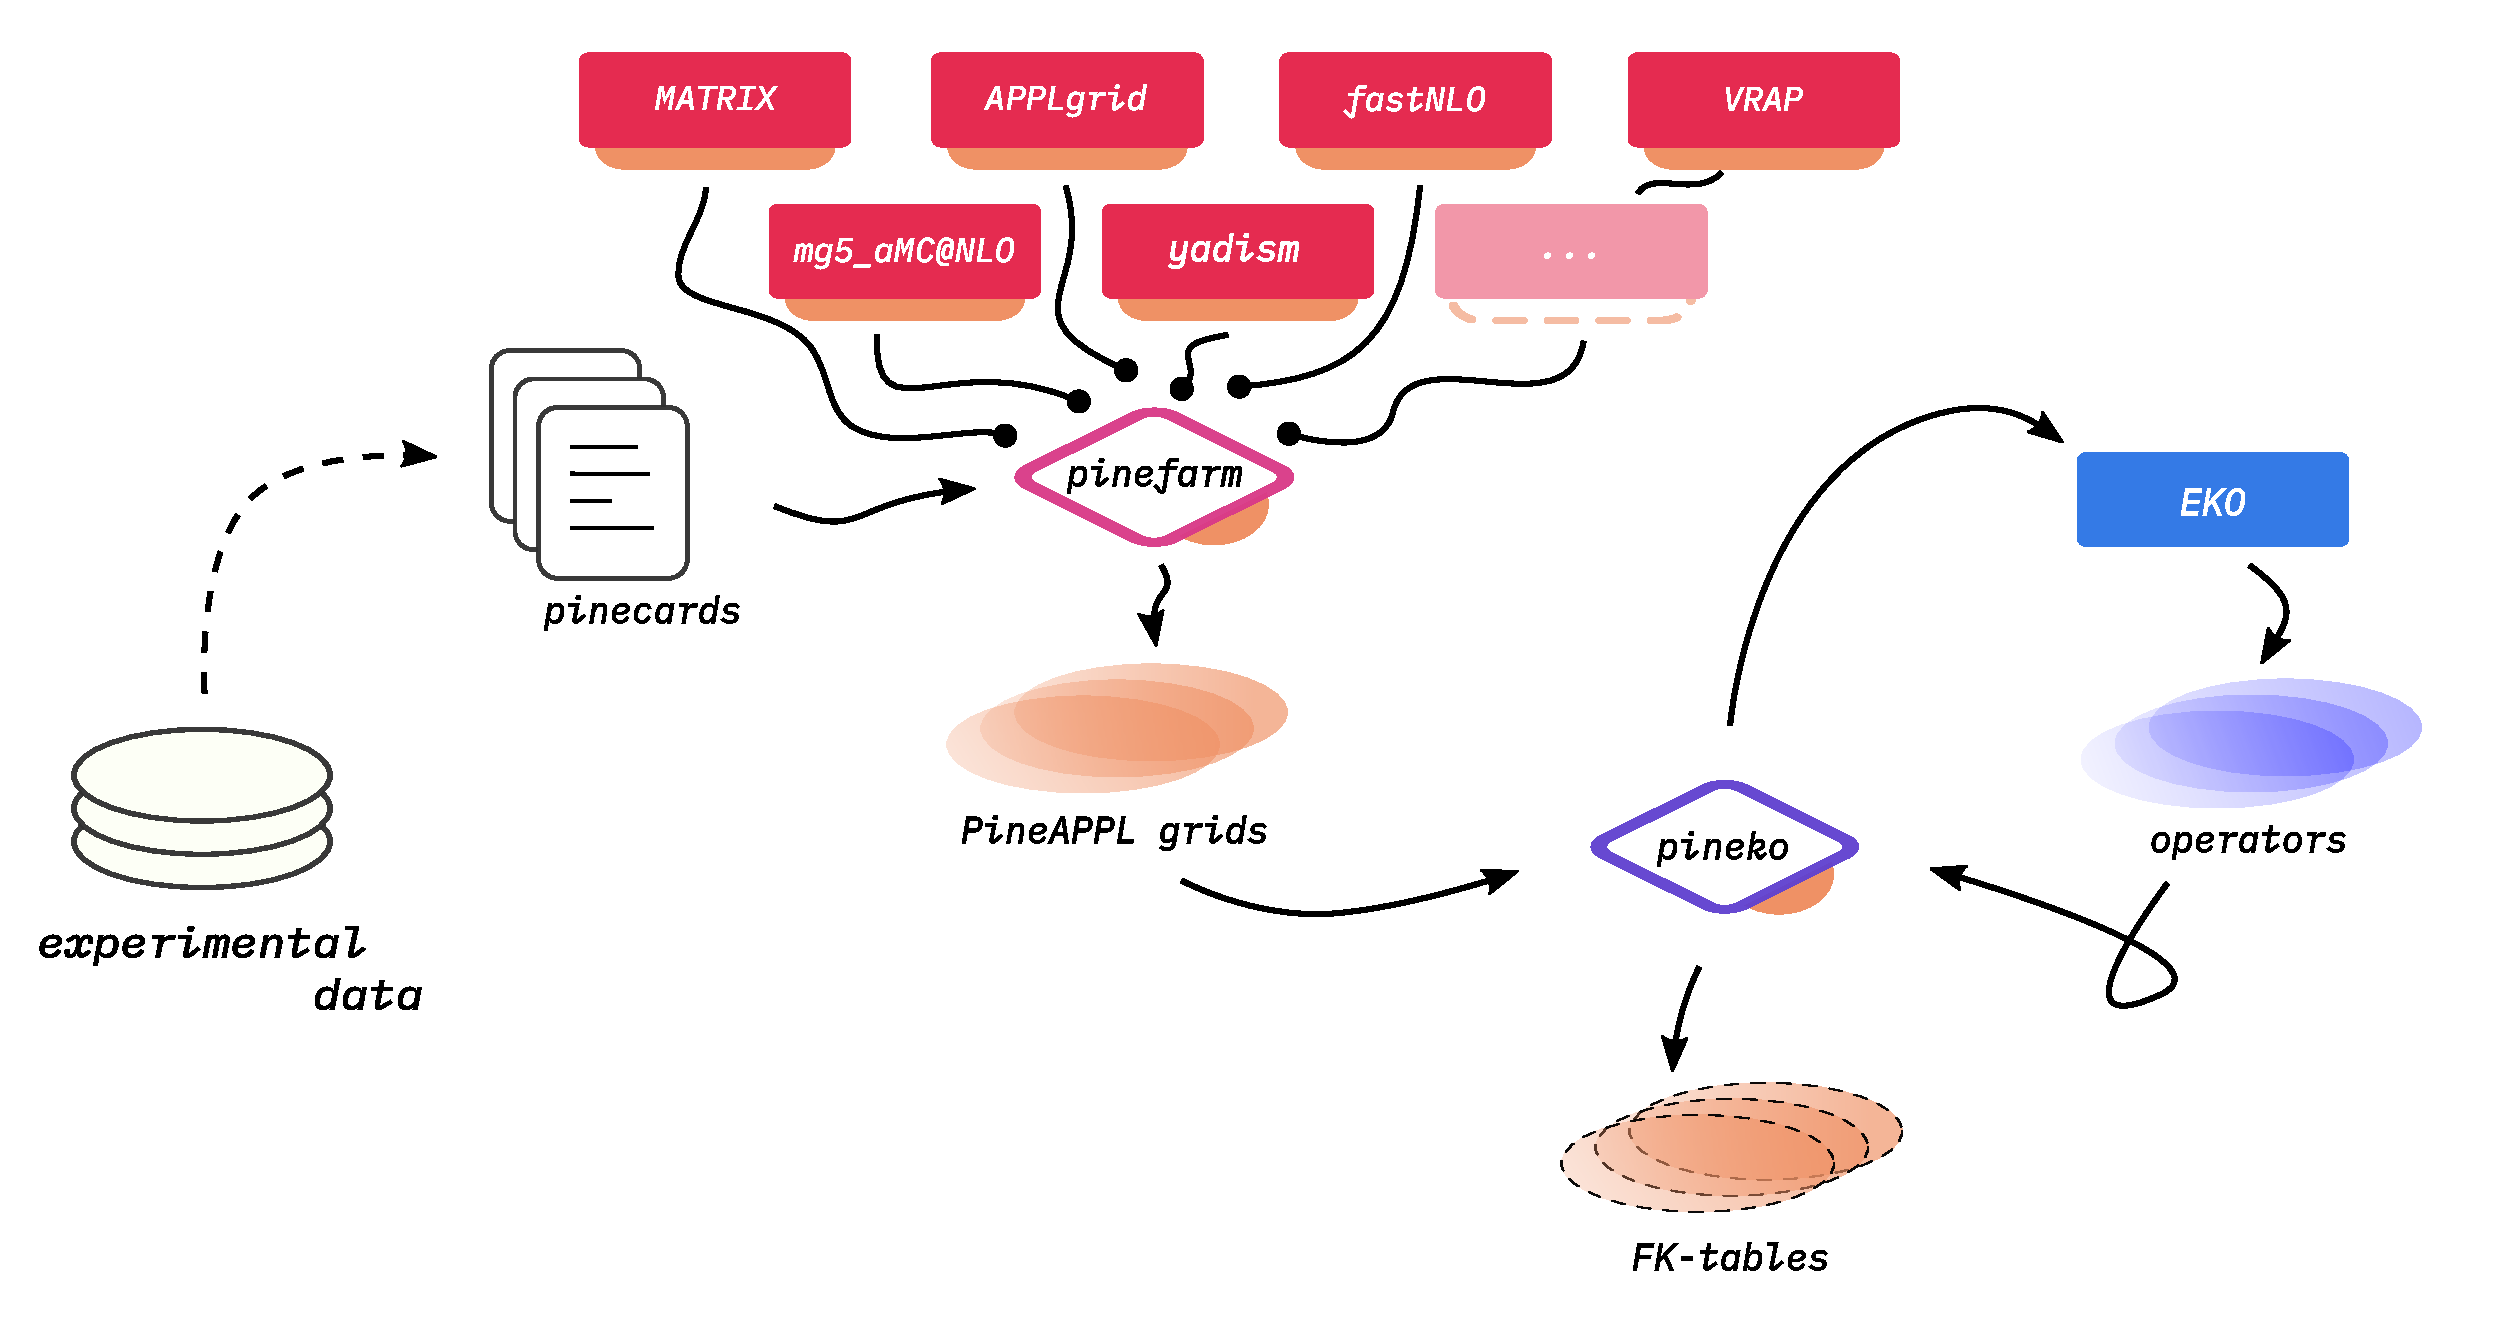
\includegraphics[width=0.9\textwidth]{ch-pineline/fk}
  \caption{
    Updated version of the flow diagram already appeared in
    \cite{Amoroso:2022eow}, showing the overall pipeline architecture.
    Arrows in the picture indicate the flow of information (together with the
    execution order), and the orange insets on other elements indicate an
    interface to \pineappl (notice \eko not having it).
    In particular, magenta blocks above \pinefarm are the providers
    \cite{Grazzini:2017mhc,Frederix:2018nkq,Carli:2010rw,candido_alessandro_2022_6285149,Britzger:2012bs,Anastasiou:2003ds}.
  }
  \label{fig:pine/pineline}
  \vspace*{-5pt}
\end{figure}

All the components of the pipeline are open source and the code is available in
the NNPDF GitHub organization:
\begin{itemize}
  \setlength\itemsep{2pt}
  \item \pineappl: \url{https://github.com/NNPDF/pineappl}
  \item \eko: \url{https://github.com/NNPDF/eko}
  \item \pineko: \url{https://github.com/NNPDF/pineko}
  \item \pinefarm: \url{https://github.com/NNPDF/runcards} (including the
    relevant pinecards, required for \nnpdf fits)
  % \item \pineappl{}grids generated - not complete, but especially the most
  %   expensive ones - \url{https://github.com/NNPDF/pineapplgrids}
  %   \fxwarning{
  %     Remove if not public: we would really shoot ourselves in the foot, since
  %     it is not needed, nor described, and definitely bad advertisement for the
  %     "all public" philosophy.
  %     But\dots is there any reason why it is private at all? Or still private?
  %   }
\end{itemize}

The set of tools does not depend
on the \nnpdf fitting methodology and can be used in general for
any hadronic function fitting\footnote{
  Generalization of \pineappl to support fragmentation functions and polarized
  \pdfs is work in progress.
}.
